\subsection{Efectos de la cuantización en procesadores digitales }

\begin{enumerate}

\item 
    Se cargan los archivos de audio \texttt{sonidos-de-voz-16-16.wav} y \texttt{musica-16-16.wav} y se desarrolla la función \texttt{cuantiza(x,N)} en MATLAB para analizar qué tanto se distorsiona una señal de audio al ser cuantizada, y cómo influyen en este proceso la cantidad de bits que se utilizan para realizar dicha cuantización.
    
    \begin{figure}[H]
        \centering
        \includegraphics[scale = 0.7]{imagenes2/cuantiza.png}
        \caption{Implementación en MATLAB de la función \texttt{cuantiza}}
        \label{fig:cuantiza}
    \end{figure}
    
    En la figura \ref{fig:cuantiza} se tiene el código de implementación para una función que cuantiza una señal que se recibe con el parámetro \textit{x}  y donde \textit{N} corresponde a la cantidad de niveles de cuantización que se considerarán en el proceso.
    
    Al realizar pruebas con distinta cantidad de bits  (para 12, 8, 4, 2 y 1 bits), y por ende, distinta cantidad de niveles de cuantización se logra concluir que el audio que más se distorsiona es  \texttt{musica-16-16.wav}. Ambos audios para una cantidades de 12 y 8 bits no sufrían notoria modificación, pero al llegar a los 4 bits se empieza a notar una significativa distorsión en el archivo de música, que aumenta en cada reducción de cantidad de bits. En el caso de el audio de sonidos de voz también se percibe deis torsión con la reducción de bits pero no era tan significativa en comparación al archivo original, aún era inteligible pero con algo de ruido, a pesar de ser cuantizada con 1 bit.Esto no ocurre con el audio de música, que con 1 bit se obtiene un audio totalmente distorsionado y casi no se distingue el audio original.
    
    
    
    \item %A continuación se observará la relación entre la percepción de escuchar de la señal cuantizada y el tipo de ruido de cuantizacón y su correlación con la señal original.
    
    \begin{enumerate}
        \item Se modifica la función cuantiza mostrada en la figura \ref{fig:cuantiza}, para que reciba los mismos parámetros de antes pero que esta vez entregue una nueva señal \textit{y} que corresponde a una cuantización de la señal original pero llevada al mismo rango de esta última. Además de entregar el error  $y-x$, donde \textit{x} corresponde a la señal original. La figura \ref{cuantiza2} muestra la implementación de la función antes descrita.
    
    
    
    \begin{figure}[H]
        \centering
        \includegraphics[scale = 0.5]{imagenes2/cuantiza2.png}
        \caption{Implementación de la función \texttt{cuantiza} modificada para entregar señal cuantizada y el error con respecto a la señal original.}
        \label{cuantiza2}
    \end{figure}
    
        
        Al aplicar esta función a los archivos de  audio \texttt{sonidos-de-voz-16-16.wav} y \texttt{musica-16-16.wav} con 4 niveles de cuantización y graficar tanto las señales originales como las cuantizadas  llevadas al mismo rango original se obtienen las gráficas presentes en la figura \ref{original_cuantizada}
        
        \begin{figure}[H]
            \centering
            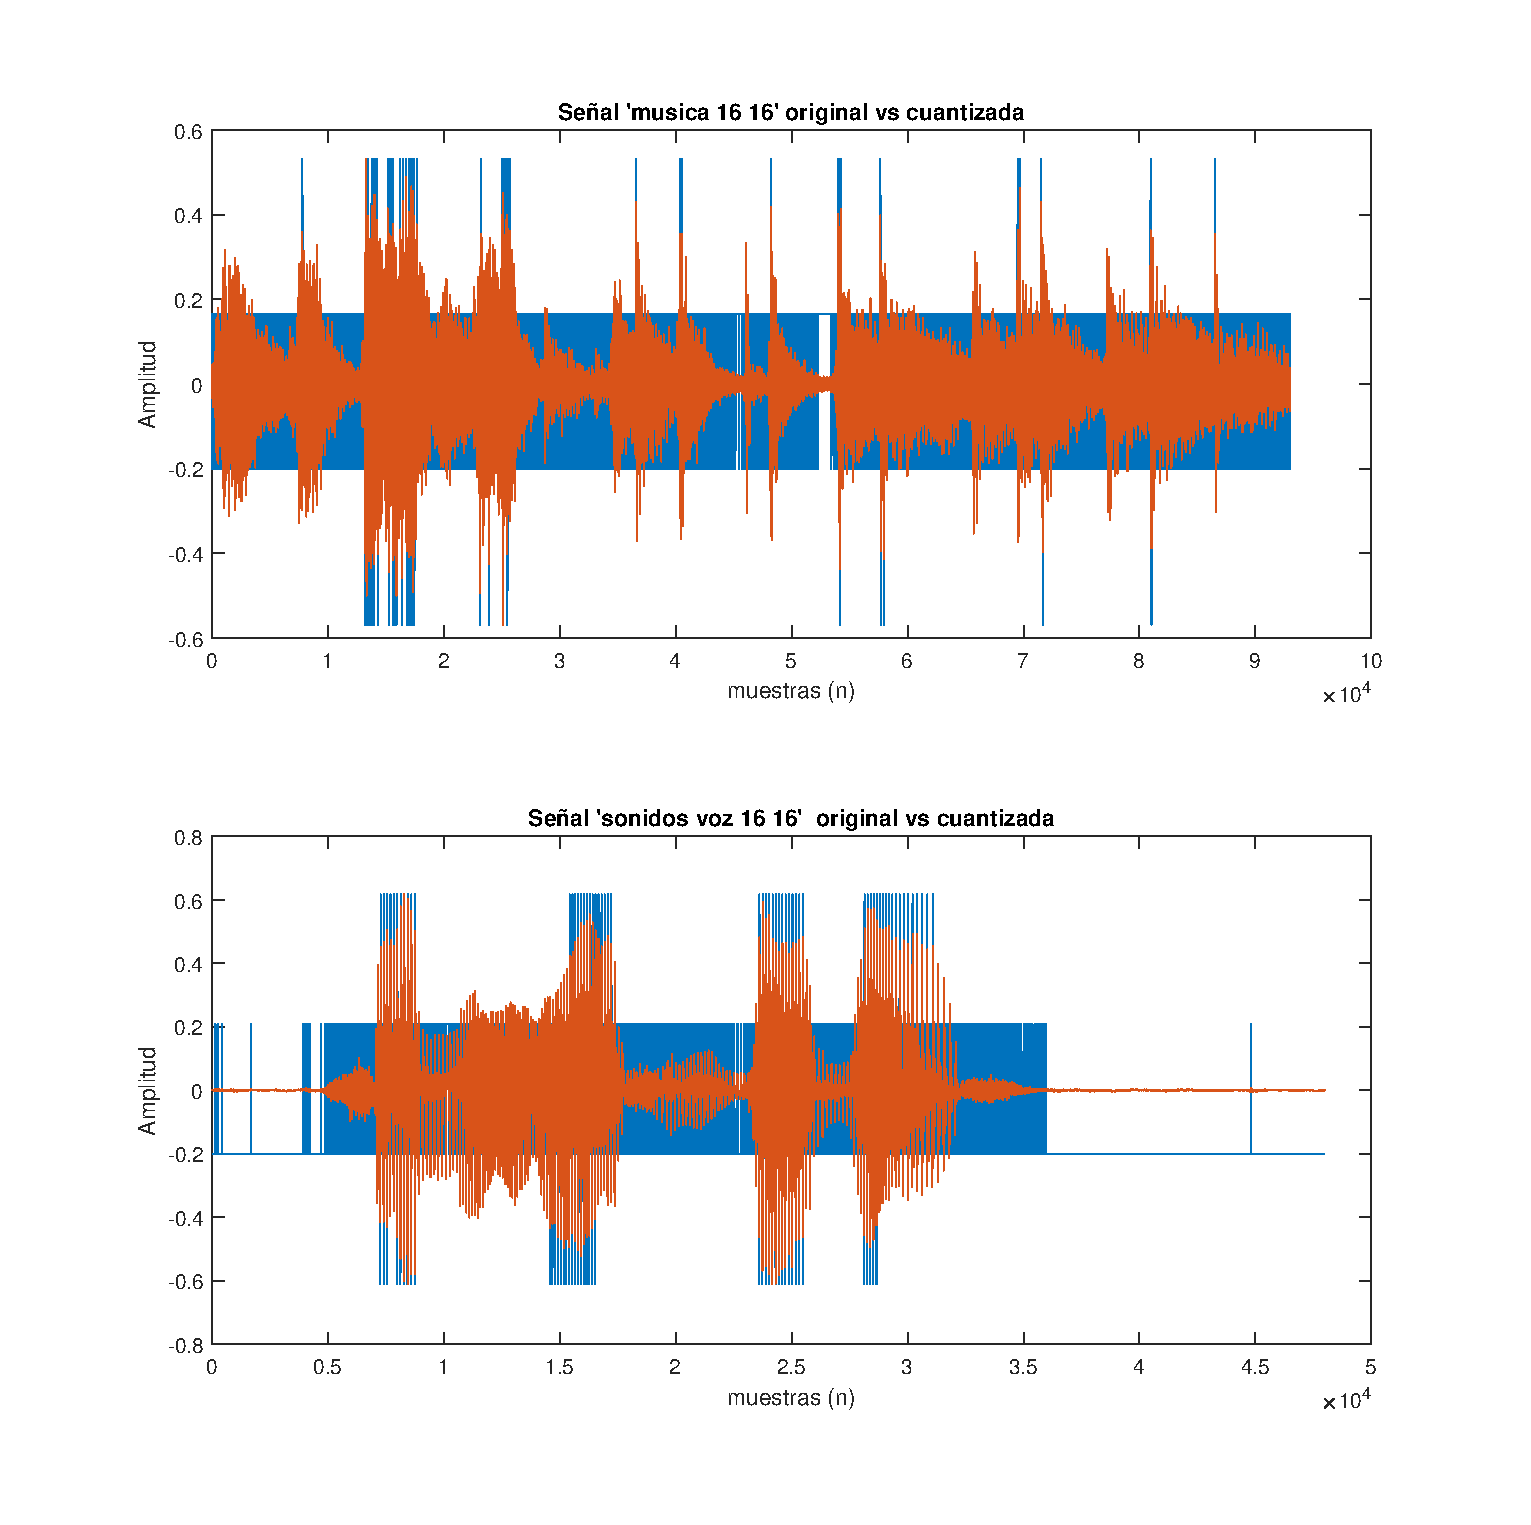
\includegraphics[scale = 0.5]{imagenes2/original_cuantizada.eps}
            \caption{Gráficas comparativas entre los archivos de audio originales y las señales obtenidas de su respectiva cuantización y reescalamiento.}
            \label{original_cuantizada}
        \end{figure}
        
  
        
        %Comentar las graficas
        
    \item Se grafican los histogramas de 20 bins del error para cada señal de audio, \texttt{musica-16-16.wav} y \texttt{sonidos-de-voz-16-16.wav}, para una cantidad de 2 bits, es decir 4 niveles de cuantización. Obteniéndose así las gráficas de la figura \ref{fig:histogramas}
    
    
    \begin{figure}[H]
        \centering
        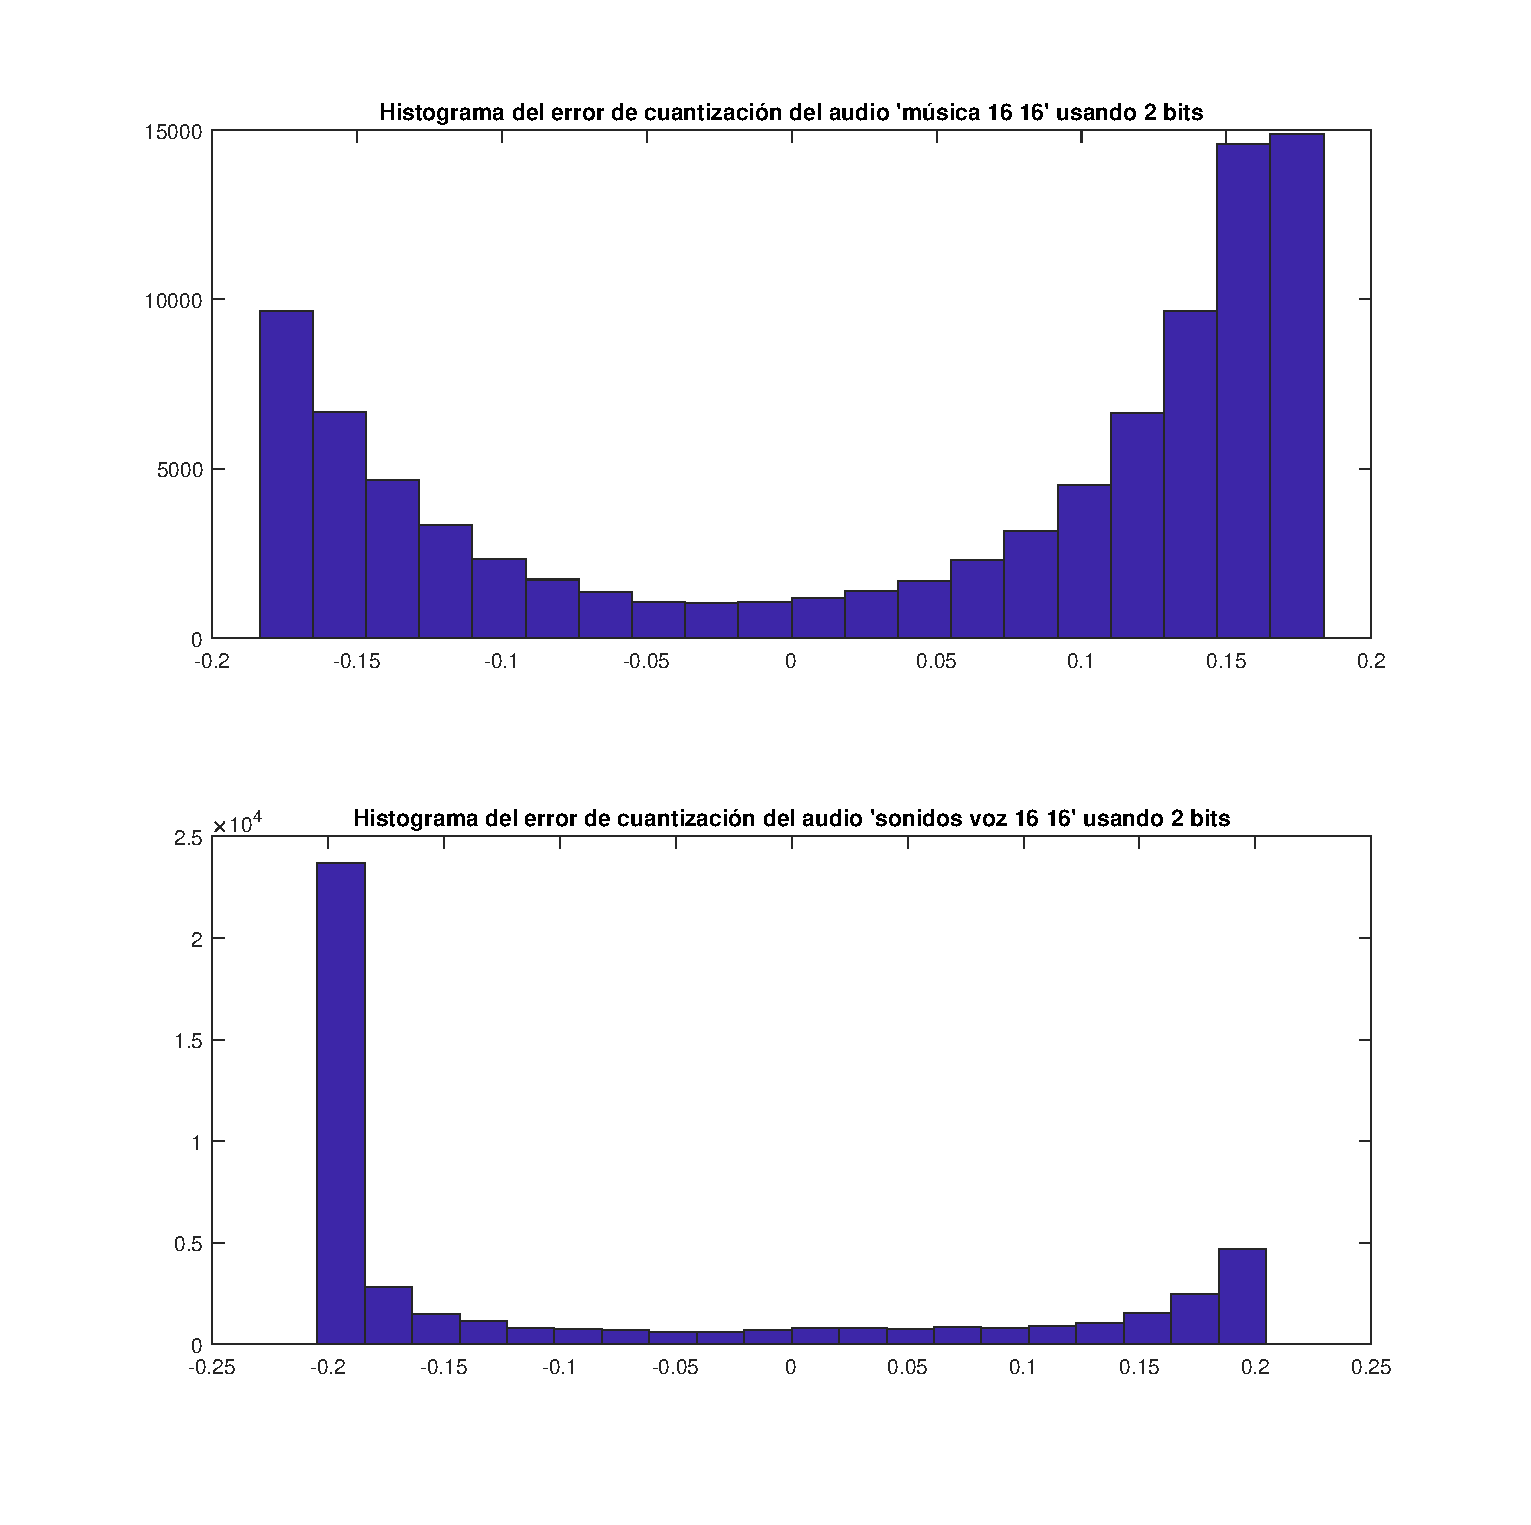
\includegraphics[scale = 0.5]{imagenes2/histogramas.eps}
        \caption{Histogramas del error asociado a la cuantización de las señales de audio  \texttt{musica-16-16.wav} y \texttt{sonidos-de-voz-16-16.wav}.}
        \label{fig:histogramas}
    \end{figure}
    
    Se realizó el proceso de graficar los histogramas del error de cuantización de las señales de audio para 1, 2, 4 , 8 y 12 y 1 bits. Se concluye que si se aumenta la cantidad de bits disponibles en la cuantización, es decir, hay más niveles de cuantización, la gráfica del histograma del error tiene  una distribución cada vez más cercana a la  uniforme,  por lo que el error  (interpretable como ruido en este caso) no está correlacionado con la señal misma. Por otro lado, al reducir la cantidad de bits disponibles, el histograma tiende a concentrarse en los extremos de las gráficas, lejos del cero. Esto es esperable ya que si hay pocos niveles de cuantización es poco probable conseguir errores de magnitud baja debido a que hay pocas opciones de valores para aproximar  el valor de la muestra, pudiendo haber mucha diferencia entre estas dos cantidades.
    
    %%%COrrelación
    \item Se obtiene la autocorrelación del error de cuantización para con diferentes cantidades de bits en el proceso (1, 2, 4, 8 y 12 bits). Además se obtiene la correlación de dicho error con la señal original, en este caso el archivo de audio \texttt{musica-16-16.wav}
    
    Las gráficas comparativas entre la autocorrelación del error de cuantización y la correlación del error con la señal original utilizando 2 y 12 bits se muestran en la figura \ref{fig:xcorr}.
\newpage    
    Con respecto a la autocorrelación del error de cuantización y la correlación con la señal original se puede comentar que:
    \begin{itemize}
        \item A medida que aumenta la cantidad de bits, la autocorrelación del error empieza a parecerse más a un delta de kronecker. Recordando que la DTFT de la autocorrelación corresponde a la Densidad Espectral de Potencia (PSD) y que la DTFT de un delta de kronecker es una constante, se concluye que el error tiene una PSD que tiende a ser plana a medida que aumentan los bits, es decir, empieza a comportarse como ruido blanco.  
        
        \item Se aprecia que al haber pocos bits existe una correlación no despreciable cuando la señal original y la señal de error tienen poco retardo entre ellas. A medida que los bits aumentan la correlación entre la señal original y el error de cuantización tiende a ser cercano a 0 aún cuando hay poco retardo. Lo anterior es un supuesto usual cuando el error corresponde a ruido blanco. 
    \end{itemize}
    
    \begin{figure}[H]
        \centering
        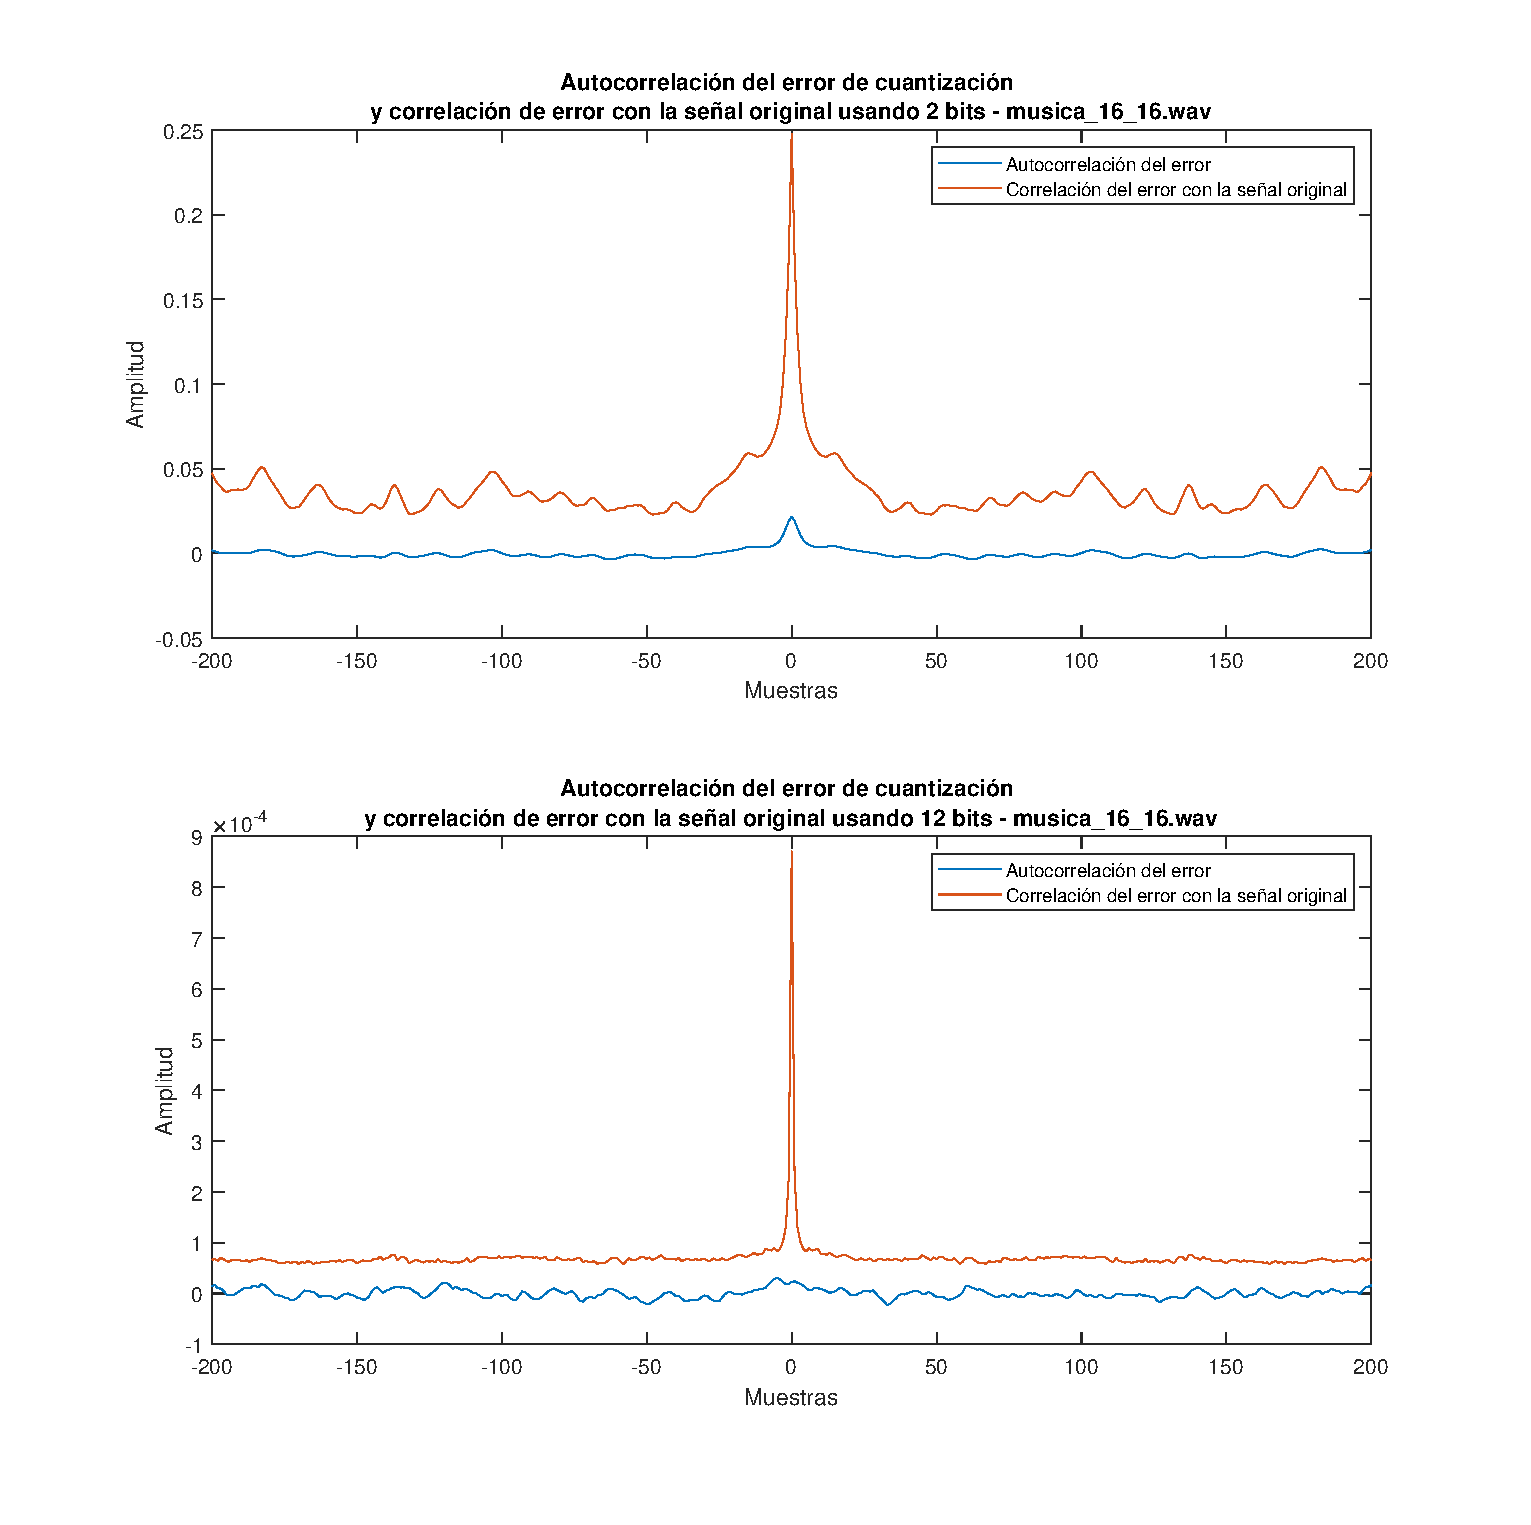
\includegraphics[width = 0.9\linewidth]{imagenes2/xcorr_error.eps}
        \caption{Autocorrelación del error de cuantización y correlación del error con la señal original para 2 y 12 bits}
        \label{fig:xcorr}
    \end{figure}
    
    
    
  \end{enumerate}
  
  
  \item Se modifica nuevamente la función para implementar \texttt{cuantiza-dither(x,N)}, que recibe los mismos parámetros que en los casos anteriores. El propósito de esta función es hacer \textit{Ditherring} a la señal para poder descorreelacionar el ruido de cuantización. Para ello se siguen pasos similares a los realizados en los casos anteriores, pero esta vez a la señal se le agrega ruido blanco o gaussiano con una desviación estándar del $25\%$ del valor de paso de cuantización. El código MATLAB que realiza esta función se encuentra en la figura \ref{dither} 
  
  
  \begin{figure}[H]
      \centering
      \includegraphics[scale = 0.5]{imagenes2/dither.png}
      \caption{Implementación en MATLAB de la función  \texttt{cuantiza-dither(x,N)}.}
      \label{dither}
  \end{figure}
  
  Al reproducir las señales obtenidas se escucha prácticamente solo ruido, a pesar de el aumento en el número de bits. En el caso de el archivo de música incluso haciendo uso de 12 bits solo se escucha ruido, para el caso del archivo de voz, usando este mismo número de bits se logra apreciar levemente el mensaje de la señal original pero de todas formas opacado casi completamente por el ruido.
  
  Comparando lo escuchado al cuantizar directamente las señales originales y lo que se obtiene al hacer la cuantización cuando se aplica \textit{Dithering}, el sonido es más inteligible al oído en el primer caso, en éste se logra notar claramente la diferencia que se produce en el resultado al modificar la cantidad de bits en la cuantización. Esto no ocurre cuando se aplica \textit{Dithering}.
  
  
    
\end{enumerate}